\documentclass[twoside]{book}

% Packages required by doxygen
\usepackage{fixltx2e}
\usepackage{calc}
\usepackage{doxygen}
\usepackage[export]{adjustbox} % also loads graphicx
\usepackage{graphicx}
\usepackage[utf8]{inputenc}
\usepackage{makeidx}
\usepackage{multicol}
\usepackage{multirow}
\PassOptionsToPackage{warn}{textcomp}
\usepackage{textcomp}
\usepackage[nointegrals]{wasysym}
\usepackage[table]{xcolor}

% Font selection
\usepackage[T1]{fontenc}
\usepackage[scaled=.90]{helvet}
\usepackage{courier}
\usepackage{amssymb}
\usepackage{sectsty}
\renewcommand{\familydefault}{\sfdefault}
\allsectionsfont{%
  \fontseries{bc}\selectfont%
  \color{darkgray}%
}
\renewcommand{\DoxyLabelFont}{%
  \fontseries{bc}\selectfont%
  \color{darkgray}%
}
\newcommand{\+}{\discretionary{\mbox{\scriptsize$\hookleftarrow$}}{}{}}

% Page & text layout
\usepackage{geometry}
\geometry{%
  a4paper,%
  top=2.5cm,%
  bottom=2.5cm,%
  left=2.5cm,%
  right=2.5cm%
}
\tolerance=750
\hfuzz=15pt
\hbadness=750
\setlength{\emergencystretch}{15pt}
\setlength{\parindent}{0cm}
\setlength{\parskip}{3ex plus 2ex minus 2ex}
\makeatletter
\renewcommand{\paragraph}{%
  \@startsection{paragraph}{4}{0ex}{-1.0ex}{1.0ex}{%
    \normalfont\normalsize\bfseries\SS@parafont%
  }%
}
\renewcommand{\subparagraph}{%
  \@startsection{subparagraph}{5}{0ex}{-1.0ex}{1.0ex}{%
    \normalfont\normalsize\bfseries\SS@subparafont%
  }%
}
\makeatother

% Headers & footers
\usepackage{fancyhdr}
\pagestyle{fancyplain}
\fancyhead[LE]{\fancyplain{}{\bfseries\thepage}}
\fancyhead[CE]{\fancyplain{}{}}
\fancyhead[RE]{\fancyplain{}{\bfseries\leftmark}}
\fancyhead[LO]{\fancyplain{}{\bfseries\rightmark}}
\fancyhead[CO]{\fancyplain{}{}}
\fancyhead[RO]{\fancyplain{}{\bfseries\thepage}}
\fancyfoot[LE]{\fancyplain{}{}}
\fancyfoot[CE]{\fancyplain{}{}}
\fancyfoot[RE]{\fancyplain{}{\bfseries\scriptsize Generated by Doxygen }}
\fancyfoot[LO]{\fancyplain{}{\bfseries\scriptsize Generated by Doxygen }}
\fancyfoot[CO]{\fancyplain{}{}}
\fancyfoot[RO]{\fancyplain{}{}}
\renewcommand{\footrulewidth}{0.4pt}
\renewcommand{\chaptermark}[1]{%
  \markboth{#1}{}%
}
\renewcommand{\sectionmark}[1]{%
  \markright{\thesection\ #1}%
}

% Indices & bibliography
\usepackage{natbib}
\usepackage[titles]{tocloft}
\setcounter{tocdepth}{3}
\setcounter{secnumdepth}{5}
\makeindex

% Hyperlinks (required, but should be loaded last)
\usepackage{ifpdf}
\ifpdf
  \usepackage[pdftex,pagebackref=true]{hyperref}
\else
  \usepackage[ps2pdf,pagebackref=true]{hyperref}
\fi
\hypersetup{%
  colorlinks=true,%
  linkcolor=blue,%
  citecolor=blue,%
  unicode%
}

% Custom commands
\newcommand{\clearemptydoublepage}{%
  \newpage{\pagestyle{empty}\cleardoublepage}%
}

\usepackage{caption}
\captionsetup{labelsep=space,justification=centering,font={bf},singlelinecheck=off,skip=4pt,position=top}

%===== C O N T E N T S =====

\begin{document}

% Titlepage & ToC
\hypersetup{pageanchor=false,
             bookmarksnumbered=true,
             pdfencoding=unicode
            }
\pagenumbering{alph}
\begin{titlepage}
\vspace*{7cm}
\begin{center}%
{\Large My Project }\\
\vspace*{1cm}
{\large Generated by Doxygen 1.8.14}\\
\end{center}
\end{titlepage}
\clearemptydoublepage
\pagenumbering{roman}
\tableofcontents
\clearemptydoublepage
\pagenumbering{arabic}
\hypersetup{pageanchor=true}

%--- Begin generated contents ---
\chapter{R\+E\+A\+D\+ME}
\label{md__r_e_a_d_m_e}
\Hypertarget{md__r_e_a_d_m_e}
homework6 of death 
\chapter{Hierarchical Index}
\section{Class Hierarchy}
This inheritance list is sorted roughly, but not completely, alphabetically\+:\begin{DoxyCompactList}
\item \contentsline{section}{main\+\_\+savitch\+\_\+14\+:\+:game}{\pageref{classmain__savitch__14_1_1game}}{}
\begin{DoxyCompactList}
\item \contentsline{section}{main\+\_\+savitch\+\_\+14\+:\+:Othello}{\pageref{classmain__savitch__14_1_1_othello}}{}
\end{DoxyCompactList}
\item \contentsline{section}{piece}{\pageref{classpiece}}{}
\end{DoxyCompactList}

\chapter{Class Index}
\section{Class List}
Here are the classes, structs, unions and interfaces with brief descriptions\+:\begin{DoxyCompactList}
\item\contentsline{section}{\mbox{\hyperlink{classmain__savitch__14_1_1game}{main\+\_\+savitch\+\_\+14\+::game}} }{\pageref{classmain__savitch__14_1_1game}}{}
\item\contentsline{section}{\mbox{\hyperlink{classmain__savitch__14_1_1_othello}{main\+\_\+savitch\+\_\+14\+::\+Othello}} }{\pageref{classmain__savitch__14_1_1_othello}}{}
\item\contentsline{section}{\mbox{\hyperlink{classpiece}{piece}} }{\pageref{classpiece}}{}
\end{DoxyCompactList}

\chapter{Class Documentation}
\hypertarget{classmain__savitch__14_1_1game}{}\section{main\+\_\+savitch\+\_\+14\+:\+:game Class Reference}
\label{classmain__savitch__14_1_1game}\index{main\+\_\+savitch\+\_\+14\+::game@{main\+\_\+savitch\+\_\+14\+::game}}
Inheritance diagram for main\+\_\+savitch\+\_\+14\+:\+:game\+:\begin{figure}[H]
\begin{center}
\leavevmode
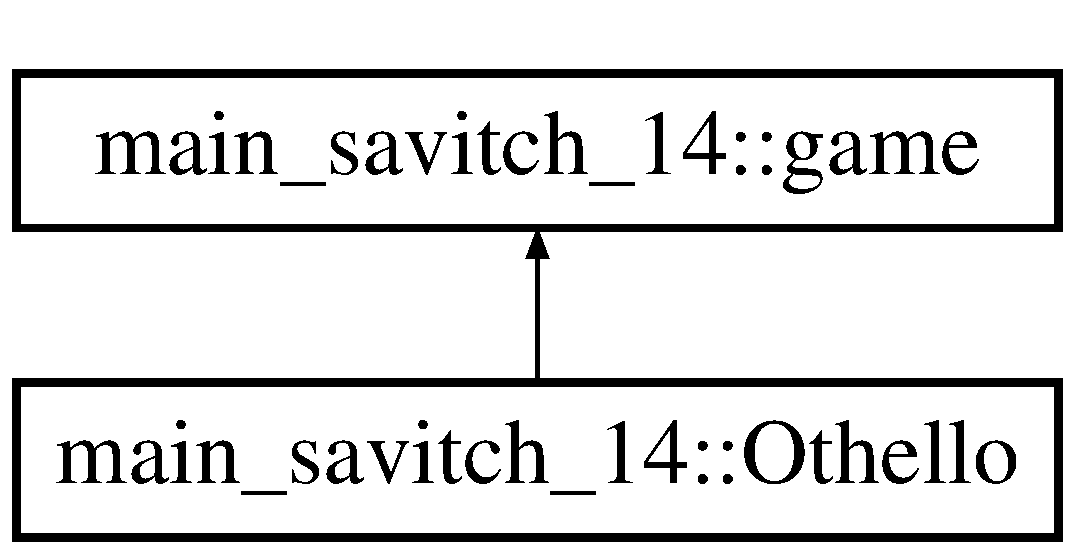
\includegraphics[height=2.000000cm]{classmain__savitch__14_1_1game}
\end{center}
\end{figure}
\subsection*{Public Types}
\begin{DoxyCompactItemize}
\item 
\mbox{\Hypertarget{classmain__savitch__14_1_1game_a4fe20fb287f809ae2b68e28e4ccba634}\label{classmain__savitch__14_1_1game_a4fe20fb287f809ae2b68e28e4ccba634}} 
enum {\bfseries who} \{ {\bfseries H\+U\+M\+AN}, 
{\bfseries N\+E\+U\+T\+R\+AL}, 
{\bfseries C\+O\+M\+P\+U\+T\+ER}
 \}
\end{DoxyCompactItemize}
\subsection*{Public Member Functions}
\begin{DoxyCompactItemize}
\item 
who \mbox{\hyperlink{classmain__savitch__14_1_1game_a4dbeaddb78059f7c5dcbf5cc4e026317}{play}} ()
\end{DoxyCompactItemize}
\subsection*{Protected Member Functions}
\begin{DoxyCompactItemize}
\item 
virtual void \mbox{\hyperlink{classmain__savitch__14_1_1game_ac58bfc07db8e604b07d2039b2cf7ab51}{display\+\_\+message}} (const std\+::string \&message) const
\item 
virtual std\+::string \mbox{\hyperlink{classmain__savitch__14_1_1game_a6504d401fcc8b138ae6342c2868c8a40}{get\+\_\+user\+\_\+move}} () const
\item 
\mbox{\Hypertarget{classmain__savitch__14_1_1game_a5c1ab8b36fb977bbe9fe387e793e4ee5}\label{classmain__savitch__14_1_1game_a5c1ab8b36fb977bbe9fe387e793e4ee5}} 
virtual who {\bfseries last\+\_\+mover} () const
\item 
\mbox{\Hypertarget{classmain__savitch__14_1_1game_a31dd5382cc6d64a6d58bcee55383cf1b}\label{classmain__savitch__14_1_1game_a31dd5382cc6d64a6d58bcee55383cf1b}} 
virtual int {\bfseries moves\+\_\+completed} () const
\item 
\mbox{\Hypertarget{classmain__savitch__14_1_1game_a4e68409618474d19742dd5f75f92f5c9}\label{classmain__savitch__14_1_1game_a4e68409618474d19742dd5f75f92f5c9}} 
virtual who {\bfseries next\+\_\+mover} () const
\item 
\mbox{\Hypertarget{classmain__savitch__14_1_1game_a98469e89e13c73a5ee70407a2164888c}\label{classmain__savitch__14_1_1game_a98469e89e13c73a5ee70407a2164888c}} 
virtual who {\bfseries opposite} (who player) const
\item 
\mbox{\Hypertarget{classmain__savitch__14_1_1game_a5954eccb6abf1ae900ad853ad2af99fa}\label{classmain__savitch__14_1_1game_a5954eccb6abf1ae900ad853ad2af99fa}} 
virtual void {\bfseries counting\+Pieces} ()=0
\item 
\mbox{\Hypertarget{classmain__savitch__14_1_1game_a98190a2bf784ce0f20533475754d136d}\label{classmain__savitch__14_1_1game_a98190a2bf784ce0f20533475754d136d}} 
virtual void {\bfseries whos\+Turn} ()=0
\item 
virtual who \mbox{\hyperlink{classmain__savitch__14_1_1game_a2f0d5338c12bd98d52fe2383ece5c45e}{winning}} () const
\item 
\mbox{\Hypertarget{classmain__savitch__14_1_1game_a20597d0caa907aea47b27fed8be3759b}\label{classmain__savitch__14_1_1game_a20597d0caa907aea47b27fed8be3759b}} 
virtual void {\bfseries make\+\_\+move} (const std\+::string \&move)
\item 
\mbox{\Hypertarget{classmain__savitch__14_1_1game_ad521a7d78e7c163a0bc28b709f0d45fd}\label{classmain__savitch__14_1_1game_ad521a7d78e7c163a0bc28b709f0d45fd}} 
virtual void {\bfseries restart} ()
\item 
\mbox{\Hypertarget{classmain__savitch__14_1_1game_a7b663057f59210dd52738facfc40d959}\label{classmain__savitch__14_1_1game_a7b663057f59210dd52738facfc40d959}} 
virtual \mbox{\hyperlink{classmain__savitch__14_1_1game}{game}} $\ast$ {\bfseries clone} () const =0
\item 
\mbox{\Hypertarget{classmain__savitch__14_1_1game_a2c0c049f5861026d0f639b5837889b7a}\label{classmain__savitch__14_1_1game_a2c0c049f5861026d0f639b5837889b7a}} 
virtual void {\bfseries compute\+\_\+moves} (std\+::queue$<$ std\+::string $>$ \&moves) const =0
\item 
\mbox{\Hypertarget{classmain__savitch__14_1_1game_ac8205178922c49bab2865187e834b726}\label{classmain__savitch__14_1_1game_ac8205178922c49bab2865187e834b726}} 
virtual void {\bfseries display\+\_\+status} () const =0
\item 
\mbox{\Hypertarget{classmain__savitch__14_1_1game_a9b9c8c5e9aa57c9a430f20b87cb047aa}\label{classmain__savitch__14_1_1game_a9b9c8c5e9aa57c9a430f20b87cb047aa}} 
virtual int {\bfseries evaluate} () const =0
\item 
\mbox{\Hypertarget{classmain__savitch__14_1_1game_a49eed20648918b03fd3e2cf78987b3d1}\label{classmain__savitch__14_1_1game_a49eed20648918b03fd3e2cf78987b3d1}} 
virtual bool {\bfseries is\+\_\+game\+\_\+over} () const =0
\item 
\mbox{\Hypertarget{classmain__savitch__14_1_1game_ad38351422ca1ee3ae58440c1c6b36b30}\label{classmain__savitch__14_1_1game_ad38351422ca1ee3ae58440c1c6b36b30}} 
virtual bool {\bfseries is\+\_\+legal} (const std\+::string \&move) const =0
\end{DoxyCompactItemize}
\subsection*{Protected Attributes}
\begin{DoxyCompactItemize}
\item 
\mbox{\Hypertarget{classmain__savitch__14_1_1game_ac4c296f4370d8e5bb5ea74b638fb827d}\label{classmain__savitch__14_1_1game_ac4c296f4370d8e5bb5ea74b638fb827d}} 
int {\bfseries move\+\_\+number}
\end{DoxyCompactItemize}


\subsection{Member Function Documentation}
\mbox{\Hypertarget{classmain__savitch__14_1_1game_ac58bfc07db8e604b07d2039b2cf7ab51}\label{classmain__savitch__14_1_1game_ac58bfc07db8e604b07d2039b2cf7ab51}} 
\index{main\+\_\+savitch\+\_\+14\+::game@{main\+\_\+savitch\+\_\+14\+::game}!display\+\_\+message@{display\+\_\+message}}
\index{display\+\_\+message@{display\+\_\+message}!main\+\_\+savitch\+\_\+14\+::game@{main\+\_\+savitch\+\_\+14\+::game}}
\subsubsection{\texorpdfstring{display\+\_\+message()}{display\_message()}}
{\footnotesize\ttfamily void main\+\_\+savitch\+\_\+14\+::game\+::display\+\_\+message (\begin{DoxyParamCaption}\item[{const std\+::string \&}]{message }\end{DoxyParamCaption}) const\hspace{0.3cm}{\ttfamily [protected]}, {\ttfamily [virtual]}}

function to display a message 
\begin{DoxyParams}{Parameters}
{\em message} & is a string passed by reference \\
\hline
\end{DoxyParams}
\mbox{\Hypertarget{classmain__savitch__14_1_1game_a6504d401fcc8b138ae6342c2868c8a40}\label{classmain__savitch__14_1_1game_a6504d401fcc8b138ae6342c2868c8a40}} 
\index{main\+\_\+savitch\+\_\+14\+::game@{main\+\_\+savitch\+\_\+14\+::game}!get\+\_\+user\+\_\+move@{get\+\_\+user\+\_\+move}}
\index{get\+\_\+user\+\_\+move@{get\+\_\+user\+\_\+move}!main\+\_\+savitch\+\_\+14\+::game@{main\+\_\+savitch\+\_\+14\+::game}}
\subsubsection{\texorpdfstring{get\+\_\+user\+\_\+move()}{get\_user\_move()}}
{\footnotesize\ttfamily string main\+\_\+savitch\+\_\+14\+::game\+::get\+\_\+user\+\_\+move (\begin{DoxyParamCaption}{ }\end{DoxyParamCaption}) const\hspace{0.3cm}{\ttfamily [protected]}, {\ttfamily [virtual]}}

function to prompt the user for their moved \begin{DoxyReturn}{Returns}
returns a string of the move the user inputted 
\end{DoxyReturn}
\mbox{\Hypertarget{classmain__savitch__14_1_1game_a4dbeaddb78059f7c5dcbf5cc4e026317}\label{classmain__savitch__14_1_1game_a4dbeaddb78059f7c5dcbf5cc4e026317}} 
\index{main\+\_\+savitch\+\_\+14\+::game@{main\+\_\+savitch\+\_\+14\+::game}!play@{play}}
\index{play@{play}!main\+\_\+savitch\+\_\+14\+::game@{main\+\_\+savitch\+\_\+14\+::game}}
\subsubsection{\texorpdfstring{play()}{play()}}
{\footnotesize\ttfamily game\+::who main\+\_\+savitch\+\_\+14\+::game\+::play (\begin{DoxyParamCaption}{ }\end{DoxyParamCaption})}

function to play the game until it is over \mbox{\Hypertarget{classmain__savitch__14_1_1game_a2f0d5338c12bd98d52fe2383ece5c45e}\label{classmain__savitch__14_1_1game_a2f0d5338c12bd98d52fe2383ece5c45e}} 
\index{main\+\_\+savitch\+\_\+14\+::game@{main\+\_\+savitch\+\_\+14\+::game}!winning@{winning}}
\index{winning@{winning}!main\+\_\+savitch\+\_\+14\+::game@{main\+\_\+savitch\+\_\+14\+::game}}
\subsubsection{\texorpdfstring{winning()}{winning()}}
{\footnotesize\ttfamily game\+::who main\+\_\+savitch\+\_\+14\+::game\+::winning (\begin{DoxyParamCaption}{ }\end{DoxyParamCaption}) const\hspace{0.3cm}{\ttfamily [protected]}, {\ttfamily [virtual]}}

function see who is winning \begin{DoxyReturn}{Returns}
returns a variable of the who class 
\end{DoxyReturn}


Reimplemented in \mbox{\hyperlink{classmain__savitch__14_1_1_othello_a4ea78b18eea66c944c0a9356349e0fd4}{main\+\_\+savitch\+\_\+14\+::\+Othello}}.



The documentation for this class was generated from the following files\+:\begin{DoxyCompactItemize}
\item 
game.\+h\item 
game.\+cc\end{DoxyCompactItemize}

\hypertarget{classmain__savitch__14_1_1_othello}{}\section{main\+\_\+savitch\+\_\+14\+:\+:Othello Class Reference}
\label{classmain__savitch__14_1_1_othello}\index{main\+\_\+savitch\+\_\+14\+::\+Othello@{main\+\_\+savitch\+\_\+14\+::\+Othello}}
Inheritance diagram for main\+\_\+savitch\+\_\+14\+:\+:Othello\+:\begin{figure}[H]
\begin{center}
\leavevmode
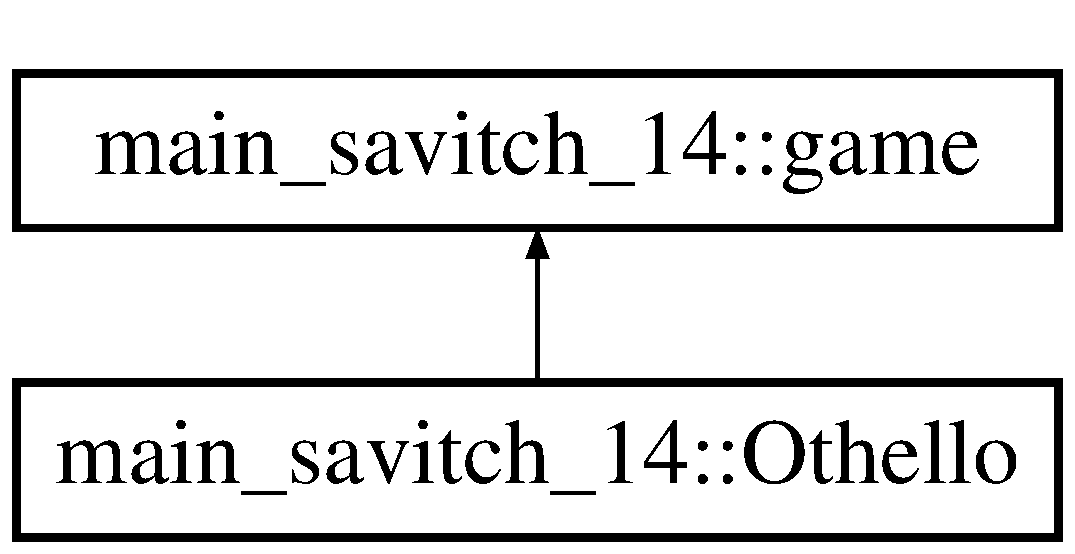
\includegraphics[height=2.000000cm]{classmain__savitch__14_1_1_othello}
\end{center}
\end{figure}
\subsection*{Public Member Functions}
\begin{DoxyCompactItemize}
\item 
\mbox{\Hypertarget{classmain__savitch__14_1_1_othello_ab01a4f7aba130133221a11224905e8ce}\label{classmain__savitch__14_1_1_othello_ab01a4f7aba130133221a11224905e8ce}} 
void {\bfseries display\+\_\+status} () const
\item 
\mbox{\Hypertarget{classmain__savitch__14_1_1_othello_a57ae44590de8d683592f186ed6bd25b0}\label{classmain__savitch__14_1_1_othello_a57ae44590de8d683592f186ed6bd25b0}} 
int {\bfseries evaluate} () const
\item 
\mbox{\Hypertarget{classmain__savitch__14_1_1_othello_a540c8b0030e429e0ac30f07e9e8868ec}\label{classmain__savitch__14_1_1_othello_a540c8b0030e429e0ac30f07e9e8868ec}} 
bool {\bfseries is\+\_\+game\+\_\+over} () const
\item 
\mbox{\Hypertarget{classmain__savitch__14_1_1_othello_a74ac0d4e6399167037dfc708efdb9033}\label{classmain__savitch__14_1_1_othello_a74ac0d4e6399167037dfc708efdb9033}} 
bool {\bfseries is\+\_\+legal} (const string \&move) const
\item 
\mbox{\Hypertarget{classmain__savitch__14_1_1_othello_a1066b280efa5cb41039585669282fe06}\label{classmain__savitch__14_1_1_othello_a1066b280efa5cb41039585669282fe06}} 
void {\bfseries make\+\_\+move} (const string \&move)
\item 
\mbox{\Hypertarget{classmain__savitch__14_1_1_othello_abf872b8074bfa4c04119317dc3b39af2}\label{classmain__savitch__14_1_1_othello_abf872b8074bfa4c04119317dc3b39af2}} 
void {\bfseries restart} ()
\item 
\mbox{\Hypertarget{classmain__savitch__14_1_1_othello_a3177234195a490eef52343d957e64b5d}\label{classmain__savitch__14_1_1_othello_a3177234195a490eef52343d957e64b5d}} 
void {\bfseries make\+\_\+skips} ()
\item 
\mbox{\Hypertarget{classmain__savitch__14_1_1_othello_a19f49edfbe82b84922877e00bc854ed8}\label{classmain__savitch__14_1_1_othello_a19f49edfbe82b84922877e00bc854ed8}} 
void {\bfseries counting\+Pieces} ()
\item 
\mbox{\Hypertarget{classmain__savitch__14_1_1_othello_a21440dbb4511812a76c578a5f546710b}\label{classmain__savitch__14_1_1_othello_a21440dbb4511812a76c578a5f546710b}} 
void {\bfseries whos\+Turn} ()
\item 
\mbox{\Hypertarget{classmain__savitch__14_1_1_othello_a7a5f8495f1a61f6e7b3968e919013c18}\label{classmain__savitch__14_1_1_othello_a7a5f8495f1a61f6e7b3968e919013c18}} 
\mbox{\hyperlink{classmain__savitch__14_1_1game}{game}} $\ast$ {\bfseries clone} () const
\item 
\mbox{\Hypertarget{classmain__savitch__14_1_1_othello_a921d4ffa277b0250f187f20b9598ebb1}\label{classmain__savitch__14_1_1_othello_a921d4ffa277b0250f187f20b9598ebb1}} 
void {\bfseries compute\+\_\+moves} (std\+::queue$<$ std\+::string $>$ \&moves) const
\item 
who \mbox{\hyperlink{classmain__savitch__14_1_1_othello_a4ea78b18eea66c944c0a9356349e0fd4}{winning}} () const
\end{DoxyCompactItemize}
\subsection*{Protected Attributes}
\begin{DoxyCompactItemize}
\item 
\mbox{\Hypertarget{classmain__savitch__14_1_1_othello_a2eed818925f68d5678b78107a3298138}\label{classmain__savitch__14_1_1_othello_a2eed818925f68d5678b78107a3298138}} 
int {\bfseries black}
\item 
\mbox{\Hypertarget{classmain__savitch__14_1_1_othello_a7d5f59b1e581ed7a8145debeecf4f310}\label{classmain__savitch__14_1_1_othello_a7d5f59b1e581ed7a8145debeecf4f310}} 
int {\bfseries white}
\item 
\mbox{\Hypertarget{classmain__savitch__14_1_1_othello_a85d4ce17512d8dbf85a313a27eea0644}\label{classmain__savitch__14_1_1_othello_a85d4ce17512d8dbf85a313a27eea0644}} 
int {\bfseries skips}
\item 
\mbox{\Hypertarget{classmain__savitch__14_1_1_othello_a15045e3e94c34afe08240885e230d502}\label{classmain__savitch__14_1_1_othello_a15045e3e94c34afe08240885e230d502}} 
int {\bfseries open\+Spots}
\item 
\mbox{\Hypertarget{classmain__savitch__14_1_1_othello_a98fbc46241d2f5e05ccb4b66f11535bf}\label{classmain__savitch__14_1_1_othello_a98fbc46241d2f5e05ccb4b66f11535bf}} 
int {\bfseries b}
\item 
\mbox{\Hypertarget{classmain__savitch__14_1_1_othello_a1b11c5fe33e30a94ed39e8cb55caf37e}\label{classmain__savitch__14_1_1_othello_a1b11c5fe33e30a94ed39e8cb55caf37e}} 
int {\bfseries w}
\end{DoxyCompactItemize}
\subsection*{Additional Inherited Members}


\subsection{Member Function Documentation}
\mbox{\Hypertarget{classmain__savitch__14_1_1_othello_a4ea78b18eea66c944c0a9356349e0fd4}\label{classmain__savitch__14_1_1_othello_a4ea78b18eea66c944c0a9356349e0fd4}} 
\index{main\+\_\+savitch\+\_\+14\+::\+Othello@{main\+\_\+savitch\+\_\+14\+::\+Othello}!winning@{winning}}
\index{winning@{winning}!main\+\_\+savitch\+\_\+14\+::\+Othello@{main\+\_\+savitch\+\_\+14\+::\+Othello}}
\subsubsection{\texorpdfstring{winning()}{winning()}}
{\footnotesize\ttfamily game\+::who main\+\_\+savitch\+\_\+14\+::\+Othello\+::winning (\begin{DoxyParamCaption}{ }\end{DoxyParamCaption}) const\hspace{0.3cm}{\ttfamily [virtual]}}

function see who is winning \begin{DoxyReturn}{Returns}
returns a variable of the who class 
\end{DoxyReturn}


Reimplemented from \mbox{\hyperlink{classmain__savitch__14_1_1game_a2f0d5338c12bd98d52fe2383ece5c45e}{main\+\_\+savitch\+\_\+14\+::game}}.



The documentation for this class was generated from the following files\+:\begin{DoxyCompactItemize}
\item 
othello.\+h\item 
othello.\+cc\end{DoxyCompactItemize}

\hypertarget{classpiece}{}\section{piece Class Reference}
\label{classpiece}\index{piece@{piece}}
\subsection*{Public Member Functions}
\begin{DoxyCompactItemize}
\item 
\mbox{\Hypertarget{classpiece_ab898c5827a5859e4cddc9d61a814a873}\label{classpiece_ab898c5827a5859e4cddc9d61a814a873}} 
void {\bfseries flip} ()
\item 
\mbox{\Hypertarget{classpiece_aa1eda7729e0f3383a813fc6ccc4e7e3c}\label{classpiece_aa1eda7729e0f3383a813fc6ccc4e7e3c}} 
bool {\bfseries is\+\_\+blank} () const
\item 
\mbox{\Hypertarget{classpiece_a103dccd216cb495d1c42b2465778be53}\label{classpiece_a103dccd216cb495d1c42b2465778be53}} 
bool {\bfseries is\+\_\+black} () const
\item 
\mbox{\Hypertarget{classpiece_ae9dde29687fcb2b7badc6cb5395a13f2}\label{classpiece_ae9dde29687fcb2b7badc6cb5395a13f2}} 
bool {\bfseries is\+\_\+white} () const
\item 
\mbox{\Hypertarget{classpiece_a31480899f2a591fdb22d97933303e19d}\label{classpiece_a31480899f2a591fdb22d97933303e19d}} 
void {\bfseries set\+\_\+white} ()
\item 
\mbox{\Hypertarget{classpiece_a273d63d07b6ea973b2fc4f7e1b56ea10}\label{classpiece_a273d63d07b6ea973b2fc4f7e1b56ea10}} 
void {\bfseries set\+\_\+black} ()
\end{DoxyCompactItemize}


The documentation for this class was generated from the following file\+:\begin{DoxyCompactItemize}
\item 
piece.\+h\end{DoxyCompactItemize}

%--- End generated contents ---

% Index
\backmatter
\newpage
\phantomsection
\clearemptydoublepage
\addcontentsline{toc}{chapter}{Index}
\printindex

\end{document}
